\documentclass[12,a4paper]{article}
\usepackage{classiccomputing}

\newcommand\postertype{lightgray}

\begin{document}

\makecclogo

\author{} % owner of the device, also used as "Author" in PDF export
\title{Wandel {\&} Goltermann IBT-10U}
\def\subtitle{ISDN Tester}
\def\introduction{Markteinführung 1996}
\makeheader{33}{40} % title size 33, subtitle size 40

%\includeimage {images/prtel93i.png}{0.5}

\makebullets{
    Land: Deutschland
}

\makemain{
    TE (Endgeräte)- und NT (Netzwerk)-Betrieb \newline
    Dienste und Bitfehlerratentest (BERT, G.821) \newline
    X.25 Test mit D und B Kanälen (X.31) \newline
    Protokollanalyse und Paketsniffing (durch PC-Interface) \newline
}

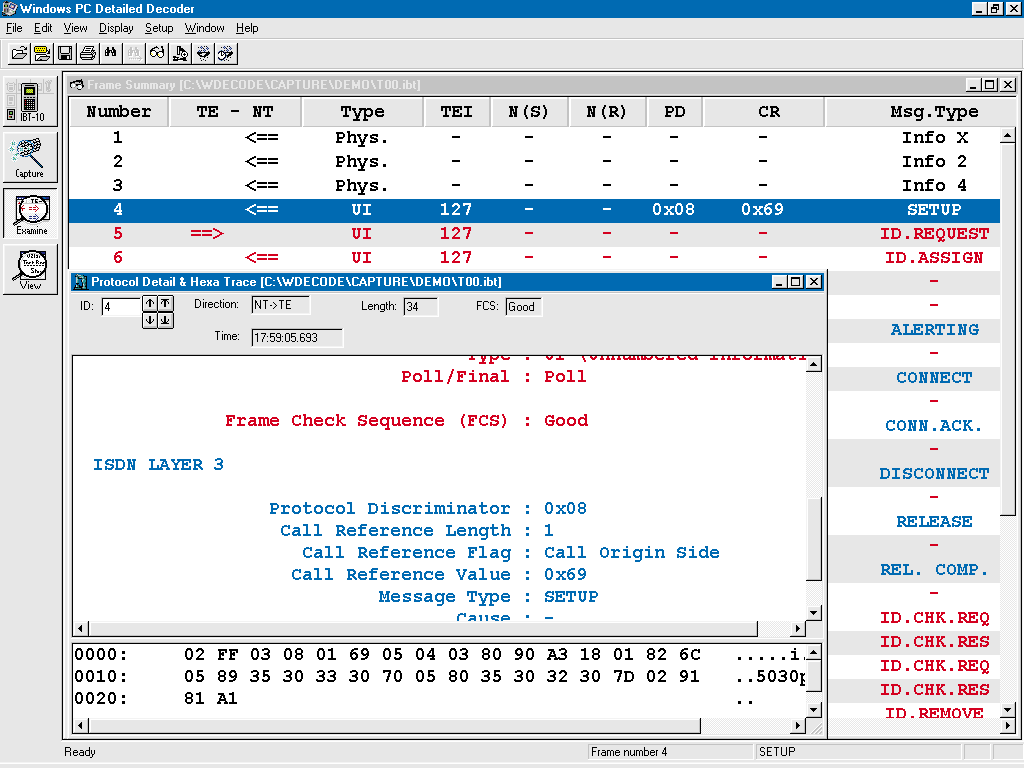
\includegraphics[width=0.7\linewidth]{images/ibt-10u.png}

\makefooter

\end{document}
